\section{实验原理}\label{section:section_3}
\subsection{取指阶段原理}
\begin{figure}[htbp]
    \centering
    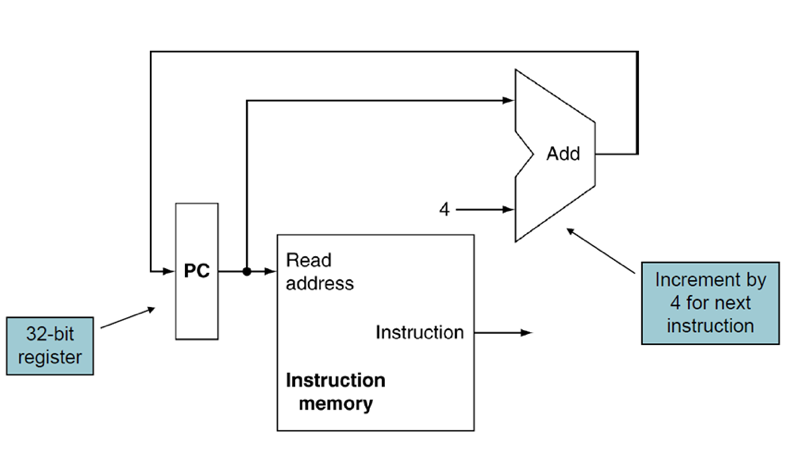
\includegraphics[width = 0.8\textwidth]{image/3_section/fetch.png}
    \caption{取指示意图}
    \label{fig:fetch}
\end{figure}

如图~\ref{fig:fetch}所示,PC为32bit(1 word)的寄存器,其存放指令地址,每条指令执行完毕后,增加4,即为下一条指令存放地址。指令地址传入指令存储器,即可取出相应地址存放的指令。
	
需要注意的是,MIPS架构中,采用字节读写,1 32bit word = 4 byte,故需要地址+4来获取下一条指令。

\subsection{指令译码原理}
\begin{figure}[htbp]
    \centering
    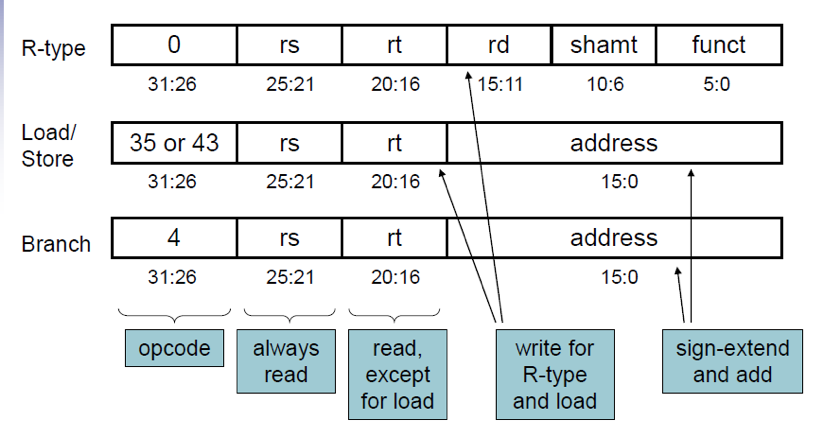
\includegraphics[width = 0.8\textwidth]{image/3_section/instruction.png}
    \caption{MIPS指令原理图}
    \label{fig:instruction}
\end{figure}
如图~\ref{fig:instruction}所示,32位MIPS指令在不同类型指令中分别有不同结构。但[31:26]表示的opcode,以及[5:0]表示的funct,为译码阶段明确指令控制信号的主要字段。表~\ref{tab:decode_sig}为opcode及funct识别得到的部分信号,详细信号表参照课本及课堂Slides。

\begin{table}[htbp]
    \centering
    \begin{tabular}{l|l|l|l|l|l}
        opcode&	aluop&	operation&	funct&	alu function	&alu control \\ \hline
        lw  &	00&	    Load word   &	XXXXXX&	Add&	010 \\ \hline
        sw  &	00&     Store word  &	XXXXXX&	Add&	010 \\ \hline
        beq &	01&	    Branch equal&	XXXXXX&	Subtact&	110 \\ \hline
        \multirow{5}{*}{R-type}& \multirow{5}{*}{10}&	Add&	100000&	qdd&	010 \\
		&   &   subtract        &	100010  &	Subtract&	110 \\
		&   &   and	            &   100100	&   And     &	000 \\
		&   &   or              &	100101  &	Or      &	001 \\
		&   &   set-on-less-than&	101010  &	SLT	    &   111 \\ \hline
    \end{tabular}
    \caption{译码控制信号}
    \label{tab:decode_sig}
\end{table}

\subsection{控制器实现原理}
\begin{figure}[htbp]
    \centering
    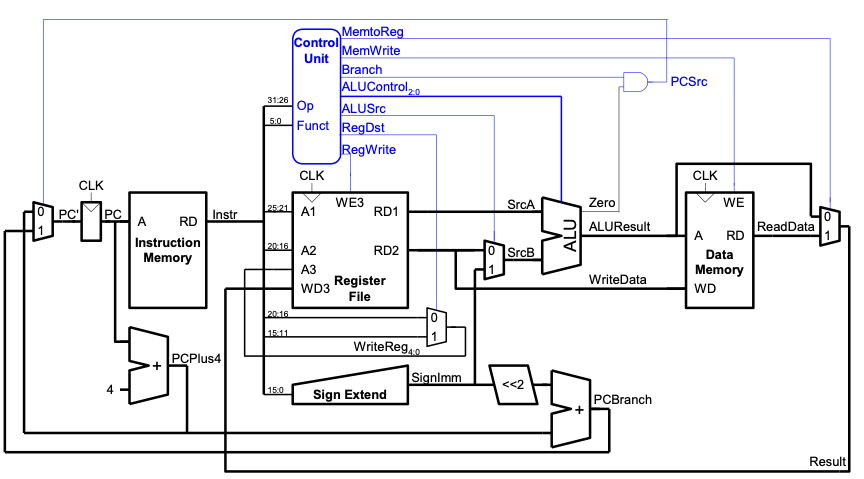
\includegraphics[width = 0.8\textwidth]{image/3_section/data_path.png}
    \caption{单周期数据通路}
    \label{fig:data_path}
\end{figure}
由图~\ref{fig:data_path}可知,控制器输出的控制信号,用于控制器件的使能和多路选择器的选择,因此,根据不同指令的功能分析其所需要的路径,即可得到信号所对应的值。在此之前,参照表~\ref{tab:sig_meaning}对各个控制信号的含义进行理解。


\begin{table}[htbp]
    \centering
    \begin{tabular}{c|c}
         信号&	含义 \\ \hline
        memtoreg&	回写的数据来自于ALU计算的结果/存储器读取的数据\\
        memwrite&	是否需要写数据存储器\\
        pcsrc&	下一个PC值是PC+4/跳转的新地址\\
        alusrc&	送入ALU B端口的值是立即数的32位扩展/寄存器堆读取的值\\
        regdst&	写入寄存器堆的地址是rt还是rd,0为rt,1为rd\\
        regwrite&	是否需要写寄存器堆\\
        branch&	是否为branch指令,且满足branch的条件\\
        jump&	是否为jump指令\\
        alucontrol&	ALU控制信号,代表不同的运算类型\\ \hline

    \end{tabular}
    \caption{信号含义}
    \label{tab:sig_meaning}
\end{table}

\newpage

分析数据通路图,判断指令是否需要写寄存器、访存等等操作,以产生相应的控制信号。下面给出参考信号表:

\begin{table}[htbp]
    \centering
    \begin{tabular}{l|l|l|l|l|l|l|l|l}
         instruction&	op5:0&	regwrite&	regdst&	alusrc&	branch&	memWrite&	memtoReg&	aluop1:0\\ \hline
        R-type&	000000&	1&	1&	0&	0&	0&	0&	10\\
        lw&	100011&	1&	0&	1&	0&	0&	1&	00\\
        sw&	101011&	0&	X&	1&	0&	1&	X&	00\\
        beq&	000100&	0&	X&	0&	1&	0&	X&	01\\
        addi&	001000&	1&	0&	1&	0&	0&	0&	00\\
        j&	000010&	0&	X&	X&	X&	0&	X&	XX \\ \hline
 
    \end{tabular}
    \caption{控制信号译码}
    \label{tab:controller_decode}
\end{table}
